% Page budget: 4 pages
\chapter{תוכנית עבודה}

\section{מבנה פירוק העבודה}
העבודה בסמסטר ב' מחולקת לחמש חבילות עבודה, שלכל אחת מהן תת־משימות ותוצר מוגדר. מבנה פירוק עבודה (\mbox{\textenglish{Work Breakdown Structure, WBS}}) מאפשר לקשור כל משימה לדרישה מפרק~2 ולבדוק אם התוצר הושג. איור~\ref{fig:ch6-wbs} מציג את המבנה ההיררכי, וטבלה~\ref{tab:ch6-wbs} מפרטת את תת־המשימות והתוצרים של כל חבילה.

\begin{figure}[h]
  \centering
  \resizebox{\textwidth}{!}{% WBS diagram: root + 5 work packages (right-to-left order, WP1 on the right).
\begin{tikzpicture}[
    root/.style={draw, very thick, rounded corners=3pt, fill=brandHighlight, minimum width=6.4cm, minimum height=0.9cm, align=center, font=\small\bfseries},
    wp/.style={draw, rounded corners=3pt, fill=paper, minimum width=2.45cm, text width=2.3cm, minimum height=2.1cm, align=center, inner sep=3pt, font=\footnotesize},
    outb/.style={draw, dashed, rounded corners=2pt, minimum width=2.45cm, text width=2.3cm, minimum height=0.9cm, align=center, inner sep=2pt, font=\scriptsize},
    ln/.style={thick, brandMain}]
  \node[root] (r) at (0,3.2) {פלטפורמת מנהל סדרה בעברית};
  \foreach \i/\x/\t/\o in {
      1/5.2/{\textbf{חבילה 1}\\ספר הסדרה ומודל הנתונים}/{ספר סדרה פעיל},
      2/2.6/{\textbf{חבילה 2}\\צוות הסוכנים והתזמור}/{צינור סוכנים},
      3/0/{\textbf{חבילה 3}\\שילוב מודלי תמונה, וידאו וקול}/{שוט עם קול וכתוביות},
      4/-2.6/{\textbf{חבילה 4}\\ממשק משתמש ומבחני שמישות}/{ממשק ודוח שמישות},
      5/-5.2/{\textbf{חבילה 5}\\בדיקות, תיעוד והגנה}/{דוח בדיקות ומצגת}} {
    \node[wp] (w\i) at (\x,0.7) {\t};
    \node[outb] (o\i) at (\x,-1.1) {\o};
    \draw[ln] (r.south) -- ++(0,-0.35) -| (w\i.north);
    \draw[ln, ->] (w\i.south) -- (o\i.north);
  }
\end{tikzpicture}
}
  \caption{מבנה פירוק עבודה: חמש חבילות עבודה}
  \label{fig:ch6-wbs}
\end{figure}

האיור מראה שהפרויקט מתפרק לחמש חבילות בלבד, כך שכל תת־משימה שייכת לחבילה אחת ואין משימה ללא תוצר. הסדר בטבלה הוא סדר הבנייה: תחילה הנתונים, אחריהם הסוכנים והמודלים, ולבסוף הממשק והבדיקות. כל תוצר נבדק מול הדרישה המתאימה מפרק~2 לפני שהחבילה הבאה נשענת עליו.

\begin{table}[h]
  \centering
  \caption{חבילות עבודה, תת־משימות ותוצרים}
  \label{tab:ch6-wbs}
  \begin{tabular}{p{2.9cm} p{5.6cm} p{3.4cm}}
    \headrow \hcell{חבילה} & \hcell{תת־משימות} & \hcell{תוצר} \\
    1. ספר הסדרה ומודל הנתונים & תכנון מבנה הנתונים של דמויות ועולם; שמירה ועדכון אחרי כל פרק & ספר סדרה פעיל \\ \rowrule
    2. צוות הסוכנים והתזמור & הגדרת תפקידי הסוכנים; חיבור ביניהם; בודק רציפות & צינור סוכנים מקצה לקצה \\ \rowrule
    3. שילוב מודלי תמונה, וידאו וקול & חיבור ספקים דרך ממשק תכנות; קול עברי; כתוביות מימין לשמאל & יצירת שוט עם קול וכתוביות \\ \rowrule
    4. ממשק משתמש ומבחני שמישות & בניית ממשק לקלט בעברית; מבחן עם משתמשים ללא רקע טכני & ממשק ודוח שמישות \\ \rowrule
    5. בדיקות, תיעוד והגנה & בדיקות מול הדרישות; תיעוד; הכנת ההגנה & דוח בדיקות ומצגת \\
  \end{tabular}
\end{table}

כל חבילה מקושרת לדרישה אחת לפחות מפרק~2. בחבילה~1 נבנה מבנה הנתונים של הדמויות והעולם, והתוצר, ספר סדרה פעיל, הוא הבסיס לבדיקת \textenglish{REQ-NAR-01}, משום שרק מצב שמור מאפשר להשוות פרק חדש לפרקים קודמים. בחבילה~2 מוגדרים תפקידי הסוכנים ובודק הרציפות, והתוצר הוא צינור מקצה לקצה; חבילה זו מאמתת את \textenglish{REQ-NAR-01} בפרקי בדיקה עם סתירות שתולות. בחבילה~3 מחוברים ספקי תמונה, וידאו וקול, והיא מאמתת את \textenglish{REQ-CHR-01} בהשוואת פנים בין סצנות, את \textenglish{REQ-LNG-01} בקול ובכתוביות בעברית ואת \textenglish{REQ-CST-01} בחישוב עלות לפי מחירוני ספקים. בחבילה~4 נבנה ממשק הקלט בעברית, ומבחן השמישות עם משתמשים ללא רקע טכני מאמת את \textenglish{REQ-UX-01}. בחבילה~5 מורצות כל הבדיקות, כולל סריקת הקוד של \textenglish{REQ-SEC-01}, ונכתבים התיעוד ומצגת ההגנה.

\section{חלוקת אחריות}
כל משימה מקבלת אחראית ביצוע אחת בלבד, והמנחה מאשר את התוצר. טבלה~\ref{tab:ch6-raci} מציגה את מטריצת האחריות (\textenglish{RACI}), שבה \textenglish{R} מבצעת, \textenglish{A} אחראית סופית, \textenglish{C} מתייעצת ואילו \textenglish{I} מעודכנת. הטבלה מראה שבכל שורה יש \textenglish{R} אחת וגם \textenglish{A} אחת, ושהמנחה הוא \textenglish{A} בכל החבילות. חלוקת התפקידים בין שתי הסטודנטיות היא הצעה ראשונית, והיא תיקבע סופית בתחילת הסמסטר.

\begin{table}[h]
  \centering
  \caption{מטריצת אחריות לפי חבילות עבודה}
  \label{tab:ch6-raci}
  \begin{tabular}{p{5.2cm} p{2.2cm} p{2.2cm} p{2.2cm}}
    \headrow \hcell{חבילה} & \hcell{סטודנטית א׳} & \hcell{סטודנטית ב׳} & \hcell{מנחה} \\
    1. ספר הסדרה ומודל הנתונים & \textenglish{R} & \textenglish{C} & \textenglish{A} \\ \rowrule
    2. צוות הסוכנים והתזמור & \textenglish{R} & \textenglish{C} & \textenglish{A} \\ \rowrule
    3. שילוב מודלי תמונה, וידאו וקול & \textenglish{C} & \textenglish{R} & \textenglish{A} \\ \rowrule
    4. ממשק משתמש ומבחני שמישות & \textenglish{C} & \textenglish{R} & \textenglish{A} \\ \rowrule
    5. בדיקות, תיעוד והגנה & \textenglish{R} & \textenglish{C} & \textenglish{A} \\
  \end{tabular}
\end{table}

\section{לוח זמנים ונתיב קריטי}
לוח הזמנים משתרע על ארבעה עשר שבועות, וקובע שתי אבני דרך, כל אחת עם שבוע רזרבה שקודם לה. תרשים גאנט (\mbox{\textenglish{Gantt chart}}) באיור~\ref{fig:ch6-gantt} מציג את משך כל חבילה, את התלויות ביניהן ואת הנתיב הקריטי, והוא נועד להראות אילו חבילות אינן יכולות להתעכב בלי לדחות את ההגשה.

\begin{figure}[h]
  \centering
  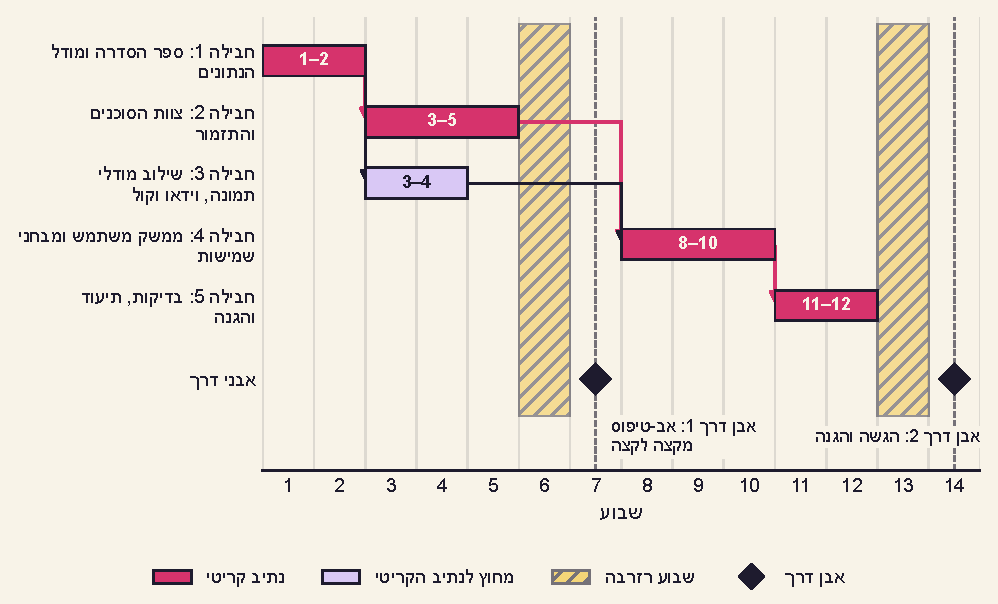
\includegraphics[width=\textwidth]{figures/ch6_gantt.pdf}
  \caption{תרשים גאנט: ארבעה עשר שבועות, נתיב קריטי ושתי אבני דרך}
  \label{fig:ch6-gantt}
\end{figure}

טבלה~\ref{tab:ch6-schedule} מסכמת את אותם נתונים במספרים: שבועות ההתחלה והסיום של כל חבילה, התלות שלה ומעמדה בנתיב הקריטי. היא מאפשרת לבדוק במבט אחד שכל חבילה מתחילה רק אחרי שהחבילות שהיא תלויה בהן הסתיימו.

\begin{table}[h]
  \centering
  \caption{לוח זמנים לפי חבילות עבודה (הערכת צוות)}
  \label{tab:ch6-schedule}
  \begin{tabular}{p{3.6cm} p{2.1cm} p{2.6cm} p{2.6cm}}
    \headrow \hcell{חבילה} & \hcell{שבועות} & \hcell{תלות} & \hcell{נתיב קריטי} \\
    1. ספר הסדרה ומודל הנתונים & \textenglish{1–2} & אין & כן \\ \rowrule
    2. צוות הסוכנים והתזמור & \textenglish{3–5} & חבילה 1 & כן \\ \rowrule
    3. שילוב מודלי תמונה, וידאו וקול & \textenglish{3–4} & חבילה 1 & לא \\ \rowrule
    4. ממשק משתמש ומבחני שמישות & \textenglish{8–10} & חבילות 2 ו־3 & כן \\ \rowrule
    5. בדיקות, תיעוד והגנה & \textenglish{11–12} & חבילה 4 & כן \\
  \end{tabular}
\end{table}

הנתיב הקריטי עובר דרך חבילה~1, חבילה~2, חבילה~4 וחבילה~5. חבילה~1 נמשכת בשבועות 1 עד 2, וחבילה~2 בשבועות 3 עד 5. אבן הדרך הראשונה בשבוע 7 היא אב־טיפוס מקצה לקצה, ושבוע 6 משמש לה רזרבה. חבילה~3 רצה במקביל לחבילה~2 בשבועות 3 עד 4, ואינה על הנתיב הקריטי, ולכן יש לה שבוע גמישות אחד. חבילה~4 נמשכת בשבועות 8 עד 10, וחבילה~5 בשבועות 11 עד 12. אבן הדרך השנייה בשבוע 14 היא הגשה והגנה, ושבוע 13 משמש לה רזרבה. משכי החבילות, התלויות ושבועות הרזרבה הם הערכת הצוות ולא נתון ממקור חיצוני, והם יעודכנו לאחר מדידת הקצב בפועל; מספר שעות העבודה השבועיות הזמינות הוא 20, כלומר שני סטודנטים כפול 10 שעות בשבוע (הנחת צוות).

לוגיקת התלויות פשוטה: חבילה אינה מתחילה לפני שהתוצר שהיא נשענת עליו מוכן. צוות הסוכנים תלוי בספר הסדרה משום שהסוכנים קוראים ממנו ומעדכנים אותו, והממשק תלוי באב־טיפוס הראשון משום שאין מה להציג לפני שהצינור פועל. חבילה~3 תלויה רק בספר הסדרה של חבילה~1, ולכן אפשר לבצע אותה במקביל לחבילה~2. הנתיב הקריטי הוא הרצף הארוך ביותר של חבילות תלויות, ולכן כל עיכוב בו מזיז ישירות את מועד ההגשה, בעוד עיכוב בחבילה~3 נספג בשבוע הגמישות שלה.

\begin{directornote}
  בפרויקט שלנו תלויות החבילות משקפות את הרעיון המרכזי: ספר הסדרה חייב להיות מוכן לפני צוות הסוכנים, ולכן עיכוב בחבילה~1 דוחה את כל הנתיב. הרזרבה בשבוע 6 נועדה לספוג בעיקר עיכוב כזה, ומבחן השמישות בחבילה~4 ייערך עם שמונה משתמשים חדשים (יעד תכנון).
\end{directornote}

\section{אבני דרך ובקרה}
בסוף כל אבן דרך נערכת בדיקה מול דרישות פרק~2. באבן הדרך הראשונה נבדקות עקביות הזהות ותפקוד הצינור מקצה לקצה, ובאבן הדרך השנייה נבדקות כלל הדרישות, כולל שמישות ועלות. אם חבילה על הנתיב הקריטי מתעכבת, שבוע הרזרבה שלפני אבן הדרך נצרך תחילה, ורק אחר כך מצומצם היקף של חבילה שאינה קריטית. כך נשמרת הגשה במועד בלי לוותר על התוצרים שהדרישות תלויות בהם. מדיניות הרזרבה קובעת שהשבוע אינו מתוכנן למשימות חדשות; הוא מנוצל רק לאחר עיכוב בפועל, ושבוע שלא נוצל משמש לתיקון ליקויים שנמצאו בבדיקה. בכל אבן דרך נערכת פגישת סקירה עם המנחה, שבה מוצג התוצר, מסומן סטטוס כל דרישה (עברה, נכשלה או טרם נבדקה) ומוחלט אם להמשיך בתוכנית או לצמצם היקף. סטייה של יותר משבוע אחד מהתכנון מדווחת למנחה באותו שבוע, וההחלטה על צמצום היקף מתועדת בטבלת הסיכונים בפרק הבא.
